\documentclass{article}

\usepackage{amsmath,amsfonts,amsthm,amssymb}
\usepackage{setspace}
\usepackage{Tabbing}
\usepackage{fancyhdr}
\usepackage{lastpage}
\usepackage{extramarks}
\usepackage{listings}
\usepackage{chngpage}
\usepackage{soul,color}
\usepackage{graphicx,float,wrapfig}
\usepackage{enumerate}
\usepackage{algorithm}
\usepackage{algorithmic}
\usepackage[english]{babel}
\usepackage[utf8]{inputenc}

\title{Spurg-Bench}
\author{Wictor Lund}

\begin{document}

\maketitle

\centerline{
\includegraphics[scale=0.4]{sb_logo.pdf}}
\vspace{20mm}

This document will give an overall description of how spurg-bench
works. The purpose of spurg-bench is to create load on a system. Since
system-wide load is a rather ambiguous concept the program is split
into replaceable components. The function of spurg-bench is to
generate multi-processable load on a multi-core system where a
load-balancer is deciding where tasks are running.

The spurg-bench test is divided into three types of components:
\begin{enumerate}
  \item The operation
  \item The load generator
  \item The runner script
\end{enumerate}

The choice of components embodies a \emph{test setup}. Spurg-bench is
designed to be an aid in development of energy efficient
load-balancing and scheduling strategies. The benchmark is not
designed to be used to create results comparable between platforms or
operating system. Another design decision is that the algorithms used
in the implementation are not simulating any particular real-world
workloads. Instead the program is designed to stress the system in a
predictive manner to test features and expose properties of the
underlying operating system.

\section{The Operation}

Spurg-bench uses an operation to generate load on a multi-core
system. The operation is usually a simple C function performing some
calculations using a CPU's computing resources such as ALU's,
floating-point unit and cache memories.

The purpose of sprug-bench is to generate a load on the system, where
the operation is the dominating type of computation. Because of the
interference caused by other processes running concurrently or in
parallel, the run time $T_{run}$ of the operation is considered
stochastic. Apart from the temporarily uncorrelated stochastic
behavior caused by interference $T_{run}$ will also be affected by the
current clock frequency. 

One should design the operation to be sufficiently short, preferably
in the length of microseconds. The operation should be short enough to
be smoothly controlled by the load generator, but at the same time be
big enough to minimize the overhead caused by the load generator. In
Listing~\ref{lst:operation} is presented an example operation which
can be used with Sprug-bench. When run on a fairly new laptop the
estimated time of this operation varies between $6$ and $11\,\mu s$,
depending on the frequency.

Generated load will consist of, even in simple cases, different types
of computation. Since different kinds of computation stresses the
system differently, a long operation with internal phases consisting
of different types of load will cause disturbing effects.

\lstset{
  language=C,
  numbers=left
}
\begin{lstlisting}[caption={Example of a operation using the processors floating-point units.},label={lst:operation}]
int operation()
{
	int	i;
	double	a  = 2.0;
	for (i = 0; i < 1000; i++) {
		a *= 2.0;
	}
	return 0;
}
\end{lstlisting}

\pagebreak
\section{The Load Generator}

The load generator runs the operation and sleeps accordingly to
generate a particular load. Since system-wide load is not very easily
defined there is a need for different load generators to enable
different definitions to be utilized.

Load generators in sprug-bench are working in phases. A phase is a
sequence of run and sleep intervals where the number of operations and
the sleep delay is constant, this is what is illustrated in
Figure~\ref{fig:run_sleep}. Phase $i$ consists of $m(i)$ sleep
intervals, each of the length $T_{sleep}(i)$\footnote{$T_{sleep}(i)$
  is a stochastic variable describing the actual sleep length, while
  $t_{sleep}(i)$ is the parameter describing how long the sleep period
  \emph{should} be.} and $n(i)\cdot m(i)$ operations each of length
$T_{run}$. The structure of a phase is illustrated with pseudo-code in
Algorithm~\ref{alg:load_gen_struct}. One should note that each
instance of $T_{sleep}(i)$ and $T_{run}$ are considered stochastic,
which means that it is impossible to calculate the total time of a
phase before it is completed. For a phase to be measurable by a system
clock, it have to be sufficiently long, but short enough to enable
fast control of the load. In practice,
should 
\begin{equation}
\label{eq:t_measure_min}
\sum_{k=1}^{m(i)}\left( T_{sleep}(i) + \sum_{l=1}^{n(i)}T_{run}
\right) > t_{measure_{min}},
\end{equation}
for some minimum measurement interval $t_{measurement_{min}}$. More
critical is that the sleep interval is long enough that the operating
system is able to cope with it.  This means that there is a
$t_{sleep_{min}}$ usually defined by the operating system or the
system clock. As mentioned, the program is structured using two nested
loops. The reason for this is to better be able to control the
real-time behaviour of the program to acheive the desired load.
\begin{enumerate}[]
\item The inner loop, looping the operation $n(i)$ times has the
  purpose of increasing the needed sleep time. Since it is possible to
  set $n(i)$ before every phase it is possible to have a minimum sleep
  time longer than $T_{run}$.
\item The outer loop, executing the inner loop and the sleep statement
  $m(i)$ times, is used to control the time between measurements. For
  optimal control performance we would need to have a constant
  measurement interval. However, due to the structure of the program
  and to the undeterministic real-time behaviour of the operating
  system this can not be achived. Instead we try to run the program
  and with adjustments to $m(i)$ achieve desired control performance.
\end{enumerate}

Due to interference it is not in general possible to run a given
number of operations and sleep a constant amount of time to retain the
reference load.

Due to interference between software processes and hardware
components, it is not in general possible to keep the parameter tuple
$\left(t_{sleep}(i), n(i), m(i)\right)$ constant for each $i$. This
has been solved by introducing a controller which estimates the time
the operation takes based earlier observations and set the sleep times
accordingly. For the estimation of $T_{run}$ it would probably be
worthwhile making the assumption that $T_{run} \propto f_{core}$,
where $f_{core}$ is the current clockfrequency of the core the load
generator is currently running on. Currently this assumption is not
being made, because of the added complexity of knowing what core the
load generator is currently running on, as well as the clockfrequency
of the current core.

The main purpose of the sleep state is to cause a context switch, and
to achieve a partial load. The context switch also causes a disruptive
behavior which severely decreases the total amount of operations per
second. In Algorithm~\ref{alg:load_gen_struct} is presented the
pseudo-code for achieving the behavior presented in
Figure~\ref{fig:run_sleep}.

\begin{algorithm}
\caption{Load generator structure}
\label{alg:load_gen_struct}
\begin{algorithmic}
  \STATE $i \leftarrow 0,\,t_{sleep}(0) \leftarrow 0,\,n(0) \leftarrow 1$
  \LOOP
  \STATE $t_{wall_1}(i) \leftarrow$ \texttt{walltime\_now()}
  \STATE $t_{cpu_1}(i) \leftarrow$ \texttt{cputime\_now()}
  \FOR{$k = 1$ to $m(i)$}
    \FOR{$l = 1$ to $n(i)$}
      \STATE \texttt{operation()}
    \ENDFOR
    \STATE \texttt{sleep($t_{sleep}(i)$)}
  \ENDFOR
  \STATE $t_{cpu_2}(i) \leftarrow$ \texttt{cputime\_now()}
  \STATE $t_{wall_2}(i) \leftarrow$ \texttt{walltime\_now()}
  \STATE
  \STATE \texttt{<< calculate $t_{sleep}(i+1)$ and $n(i+1)$ >>}
  \STATE
  \STATE $i \leftarrow i + 1$
  \ENDLOOP
\end{algorithmic}
\end{algorithm}

\begin{figure}
  \centerline{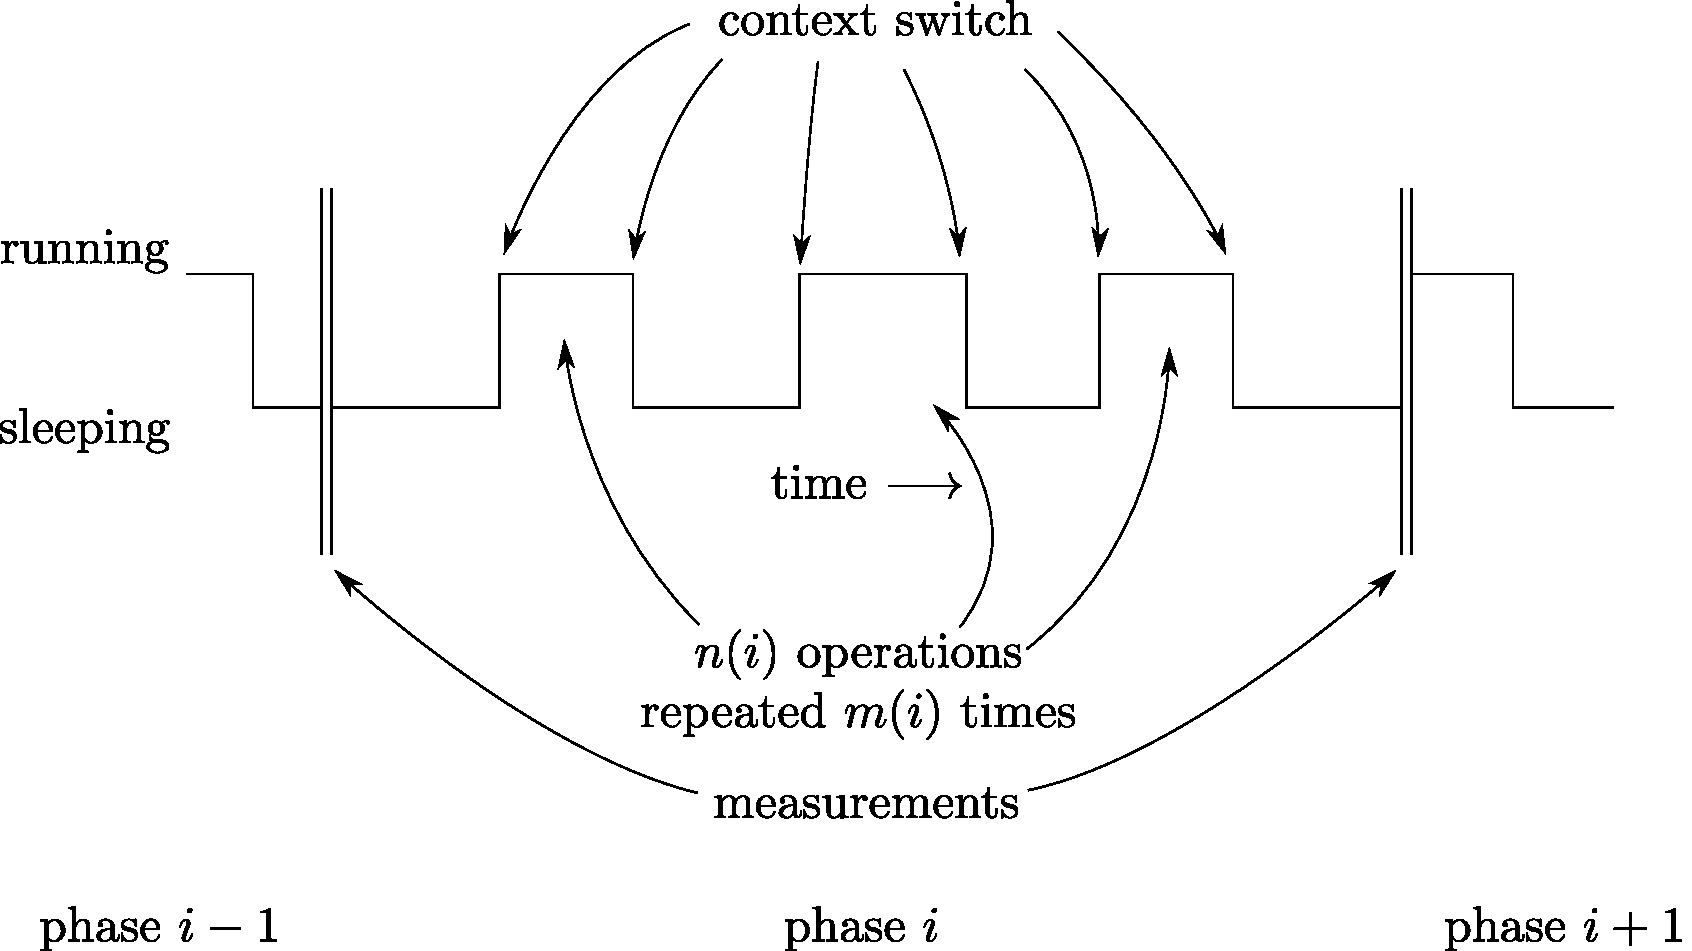
\includegraphics[scale=0.4]{run_sleep.pdf}}
  \caption{Illustration of a phase in a load generator, with it's
    context-switches, $m(i)$ sleep intervalls and $m(i)\cdot n(i)$
    operations.}
  \label{fig:run_sleep}
\end{figure}

\subsection{Load with \texttt{rusage} as the reference}

The control algoithm will take the \texttt{cpu\_time} and
\texttt{wall\_time} deltas, $$\Delta
t_{cpu}(i)=t_{cpu_2}(i)-t_{cpu_1}(i)$$ and $$\Delta
t_{wall}(i)=t_{wall_2}(i)-t_{wall_1}(i),$$ as input and give $m(i+1)$,
$n(i+1)$ and $t_{sleep}(i+1)$ as output. Internally the algorithm will
estimate the time it takes to run an operation $t_{run}(i)$. This
estimation is made using a moving average with the formula
$$\hat{t}_{run}(i+1)=\alpha\cdot\frac{\Delta t_{cpu}(i)}{m(i)\cdot n(i)}+
(1-\alpha)\cdot t_{run}(i),$$ where $\alpha$ is a exponential back-off
contant\footnote{The value for $\alpha$ which has been used is $0.5$.}.

Using this algorithm the model for the load is given
as $$L(i)=\frac{n(i)\cdot t_{run}(i)}{t_{sleep}(i) + n(i)\cdot
  t_{run}(i)}.$$ This definition of load is very comparable to the
load \texttt{top} gives, when $t_{sleep}(i)+n(i)\cdot t_{run}(i)=1s$
and \texttt{top}'s delay is set to $1s$.

If now know the target load $L(i)$ and have the estimated operation
time $\hat{t}_{run}(i)$, we can now derive an expression for the next
sleep interval length $t_{sleep}(i+1)$ using the definition of load,
and the fact that $t_{sleep}(i) \geq t_{sleep_{min}} \forall i$. The
load definition gives the inner loop length $$n(i) =
\frac{L(i)}{L(i)-1}\cdot\frac{t_{sleep}(i)}{t_{run}(i)}.$$ If we now
insert $t_{sleep}(i) \geq t_{sleep_{min}} \forall i$ into the equation
and let $n(i)$ be the smallest integer bigger than required and also
assume $t_{run}(i)\approx\hat{t}_{run}(i)$, we will get $$
n(i)=\left\lceil
\frac{L(i)}{L(i)-1}\cdot\frac{t_{sleep_{min}}}{\hat{t}_{run}(i)}
\right\rceil.$$ We can now calculate the sleep interval $t_{sleep}(i)$
using the load definition and the above assumption with
 $$t_{sleep}(i)=\frac{L(i)-1}{L(i)}\cdot \hat{t}_{run}(i)\cdot n(i).$$




\subsection{Load with operations per second as the reference}

Load generator which regulates load with operations per second as a
reference.

\section{The Runner Script}

The runner script starts up several load generators to create
multi-processing load.

\end{document}

%%  LocalWords:  sprug
